\chapter{Motivating Scenarios}
\label{chap:examples}

\section{Finding Business Addresses}
Finding a company's address or correcting an address is a common scenario that crowdsourcing is popularly applied. In the following two different cases for this scenario are exemplified and implemented.

Let's assume that we have a list of companies. The list contains company names and their corresponding mailing and website addresses. However, the mailing addresses change when company moves or names are updated. Also web addresses can change too. What we want to do is employ people to check company websites and extract address information and update their address if it is altered.

The company list is input to the application and processed by human workers. Finally, results are saved into a file. This is presented in Figure~\ref{fig:scenario1} and detailed in the following operator by operator:

\begin{figure}[ht]
	\centering
	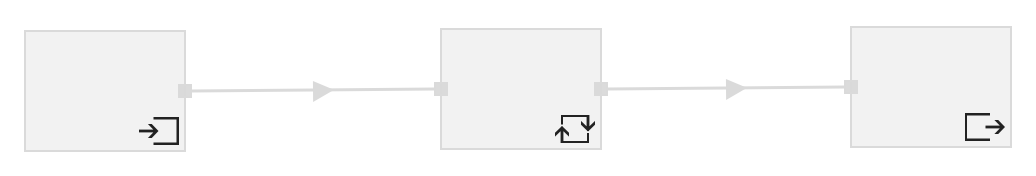
\includegraphics[width=0.85\textwidth]{figures/scenarios/naive.png}
	\caption{Crowdy application to correct business addresses.}
	\label{fig:scenario1}
\end{figure}

\textbf{source manual operator.}
Source manual operator is supplied with company list and the delimiter is selected to be comma. A small part of the list is displayed in Figure. This operator outputs the data tuples in which there are company, website and mail segments.

%input: N/A
%output: {company: company name, website: company's website address, mail: company's mailing address}

\textbf{human processing operator.}
Human processing operator gets data tuples from the source operator. Tuples are used to create the question and ask human workers to check website and mailing addresses. Workers are allowed to work on the task at most 5 minutes and they are given \$0.10 per successful completion.

Figure displays the question that is shown to human workers.

%input: {company: company name, website: company's website address, mail: company's mailing address}
%output: {company: company name, updated_website: company's updated website address, updated_mail: company's updated mailing address}

\textbf{sink operator.}
Sink file operator receives updated information per company and saves them into a file.

%input: {company: company name, updated_website: company's updated website address, updated_mail: company's updated mailing address}
%output: N/A


Different than the previous solution, we can follow 

- Human ask if updated
- Split
- Email


\section{Translation}
Translation is one of the scenarios that crowdsourcing platforms are being challenged. This scenario is complex, challenging, time-consuming and highly subjective. It cannot be easily solved by typical human tasks, because tasks are interdependent and parallel approach would not work well on such a scenario.

The overall problem that we are trying to solve is to translate a Turkish poem to English using Crowdy platform. The input to the application is the famous poet Rumi's poem "Etme" (shown in Figure~\ref{fig:scenario2.poem}) and we expect to get a translated version of it as an output. In the following, a Crowdy application  is created to translate this poem into English. The application is improved progressively over a couple of iterations.

\begin{figure}[ht]
	\centering
	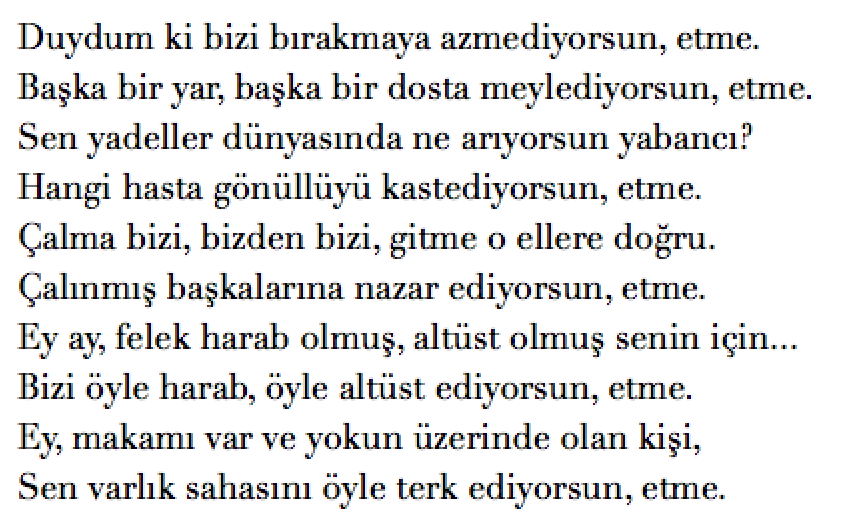
\includegraphics[height=125px]{figures/scenarios/poem.png}
	\caption{Some part of Rumi's Poem "Etme".}
	\label{fig:scenario2.poem}
\end{figure}

\subsection{Naive Approach}
The naive approach to solve this problem would be inputing the poem into the application line by line, and asking people to translate a line, and finally saving results into a file. This approach is demonstrated in Figure~\ref{fig:scenario2} and detailed in the following operator by operator:

\begin{figure}[ht]
	\centering
	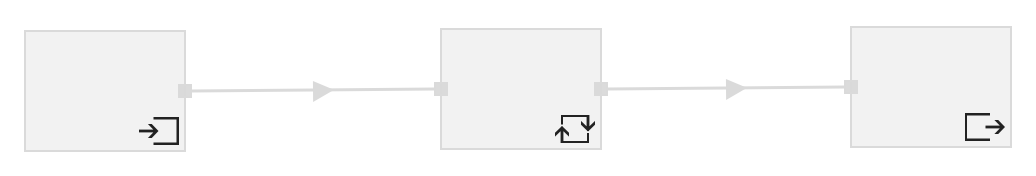
\includegraphics[width=0.85\textwidth]{figures/scenarios/naive.png}
	\caption{Crowdy application to translate a text.}
	\label{fig:scenario2}
\end{figure}

\textbf{source manual operator.}
Source manual operator is supplied with the poem and the delimiter is selected to be none. Some portion of the poem is displayed in Figure. This operator outputs the data tuples in which there is one segment called "line" and a line from the poem for the corresponding segment.

%input: N/A
%output: {line: a line from poem}

\textbf{human processing operator.}
Human processing operator gets data tuples from the source operator. Tuples are used to create the question and ask human workers to do the translation. Workers are allowed to work on the task at most 5 minutes and they are given \$0.10 per successful completion.

Figure presents a sample question that is shown to human workers.

%input: a line from poem
%output: {line: a line from poem, translation: translated line}

\textbf{sink operator.}
Sink file operator receives a line from the poem with it's translated version and saves that into a file.

%input: {line: a line from poem, translation: translated line}
%output: N/A

\subsubsection{Issues}
This approach takes the poem and employ human workers for translation. There is no quality control. Therefore, low quality assignments are possible and would probably affect the overall result.

Another issue is that the order of tuples received by sink operator is going to be probably different than the actual order. The time that human task is assigned to a worker and the duration that takes for human worker to complete that task cannot be known, although max time allotted to complete the task is set by requester. Thus, there is no guarantee that the human tasks are picked up and completed in order. The file that is created and filled by sink operator the lines from the poem will be in a random order.

\subsection{A More Sophisticated Approach}
The naive approach can be improved by adding an extra segment in the source operator and a utility operator, specifically sort operator, as shown in Figure~\ref{fig:scenario2.1}. In that way, some of the issues pointed out in the previous iteration are resolved.

\begin{figure}[ht]
	\centering
	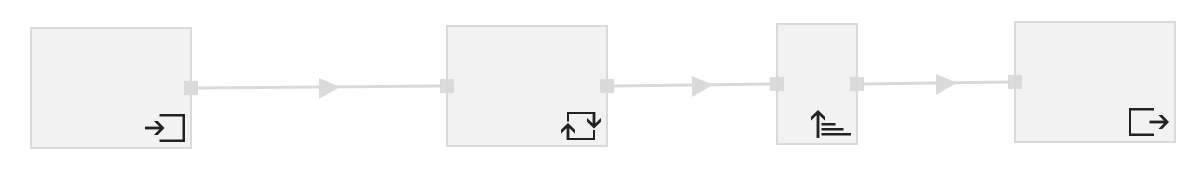
\includegraphics[width=0.85\textwidth]{figures/scenarios/scenario2_1.png}
	\caption{Crowdy application to translate a text.}
	\label{fig:scenario2.1}
\end{figure}

The input in source operator is updated by adding line numbers to the lines. The input corresponding to the one given in the previous iteration (Figure ~\ref{fig:scenario2.poem}) is displayed in Figure~\ref{fig:scenario2.poem2}. Line numbers are separated by tabs, so now the delimiter is selected to be a tab.

\begin{figure}[ht]
	\centering
	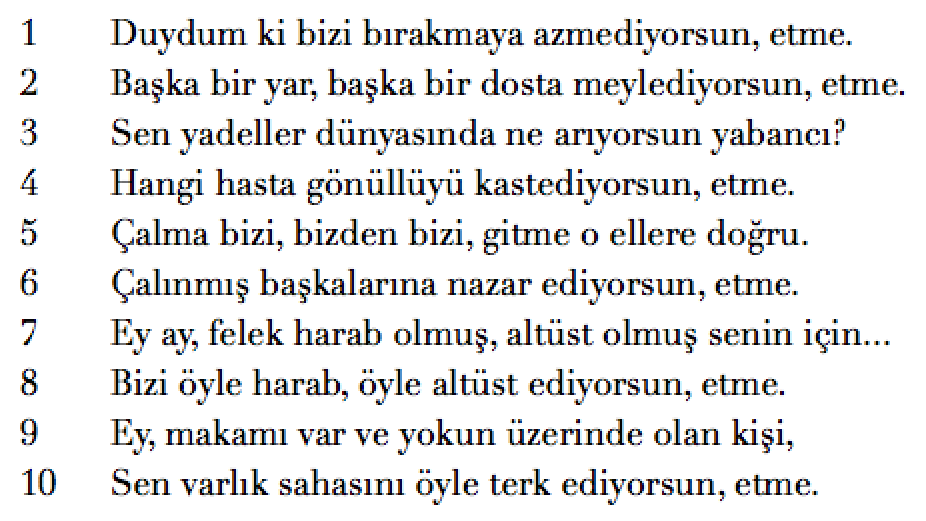
\includegraphics[height=125px]{figures/scenarios/poem2.png}
	\caption{Some part of Rumi's Poem "Etme".}
	\label{fig:scenario2.poem2}
\end{figure}

In addition, sort operator is added to the application in between human operator and sink operator. This operator takes the translate lines from human operator and sorts them with respect to line numbers. The window size of sort operator is set to the number of lines in the poem, so that sorting is done once all the lines are translated. Therefore, the sink operator receives the lines in the order they are given in the poem.

\subsubsection{Issues}
Quality control is still the problem for the new approach. The translation done by human workers is not guaranteed to have a good quality. Therefore, quality control is a fundamental requirement.

\subsection{Final Approach}
In this approach, quality control is added to the application. Figure~\ref{fig:scenario2.2} demonstrates the application created in the final approach.

\begin{figure}[ht]
	\centering
	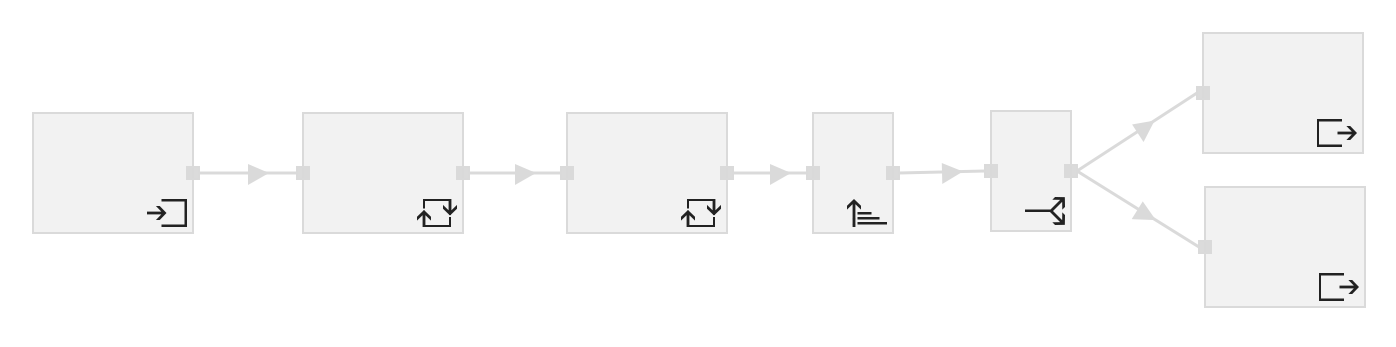
\includegraphics[width=0.85\textwidth]{figures/scenarios/scenario2_2.png}
	\caption{Crowdy application to translate a text.}
	\label{fig:scenario2.2}
\end{figure}

The output from human operator is connected to another human operator that asks people to evaluate the translation done by others. The output from this operator has an extra segment that provides the condition indicating whether translation seems OK or not. Figure shows the question shown to human workers.

Additionally a split operator can be placed before sink operator. This operator can take a data tuple and check if it has a good quality translation or not. Using this condition translated lines can be separated into two files. In this way, requesters are able to see which lines are translated well, which are not.

\subsubsection{Issues}
The issues related to quality control are resolved. However, the reliability of this solution can be still questioned, since people are employed to check the quality of the work done by other people. This issue is further discussed in Chapter~\ref{chap:discussion}.